\documentclass{article}
\usepackage[utf8]{inputenc}
\usepackage[english,vietnamese]{babel}
\usepackage{graphicx}
\usepackage{hyperref}

\title{Distributed System\\
       Practical Work 3: MPI File Transfer}
\author{Group 1}
\date{\today}

\begin{document}
\selectlanguage{english}
\maketitle

\section{Design}
For this practical we used \href{https://mpi4py.readthedocs.io}{mpi4py}
as the Python binding for MPI, which is implementation independent.
The group members choose to use MPICH to run the program because it is available
on the majority of GNU/Linux distributions.

The service was designed as a simplified version of the RPC file transfer.
\begin{center}
  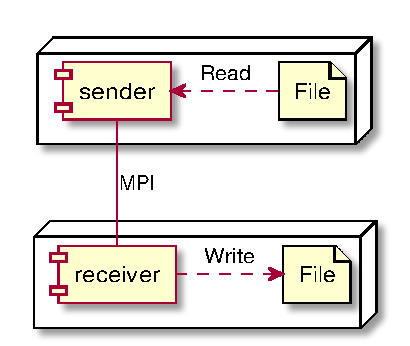
\includegraphics[width=0.5\textwidth]{mpi/arch.pdf}
\end{center}

Unlike the RPC file transfer, file discovery was not considered
due to the difficulties of setting up MPI across different machines
for it for be useful.

The file system was organized as follows:
\begin{center}
  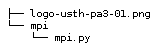
\includegraphics[width=0.5\textwidth]{mpi/files.pdf}
\end{center}
\pagebreak

\section{Implementation}
The MPI communication was set up as follows:
\begin{verbatim}
from mpi4py import MPI

comm = MPI.COMM_WORLD
rank = comm.Get_rank()
\end{verbatim}

The process of rank 0 was then used for sending the file,
which was solely passing the binary data to \verb|send|:
\begin{verbatim}
if (rank == 0):
    f = open("../logo-usth-pa3-01.png", "rb")
    data = f.read()
    comm.send(data, dest=1)
\end{verbatim}

The process of rank 1 was used for receiving the file,
which was solely writing the binary data from \verb|recv| to disk:
\begin{verbatim}
elif (rank == 1):
    data = comm.recv(source=0)
    f = open("logo.png", "wb")
    f.write(data)
\end{verbatim}

\section{Credits}
The MPI file transfer was designed and implemented
by {\selectlanguage{vietnamese}Ngô Xuân Minh}, and this article was written
by {\selectlanguage{vietnamese}Nguyễn Gia Phong}.
\end{document}
